\chapter{Estat actual}
\label{cap:estat}


% * Sèries temporals
  
%   - mineria
%   - aplicacions
%   - monitoratge de sèries temporals i problemes
%      * censura
%      * mostreig

%   - sgst: 
%       ficar aquí els sgbd per sèries temporals i més endavant ja es parlarà dels sgbd en general i com modelar-los i implementar-los.


% * SGBD
%  - model relacional
%  - implementacions
%  - temporal data


  % * Sèries temporals (històrics, predicció, diagnosis, prognosis, etc.)
  % * Mostreig: docs quan període de mostreig no regular
  % * Bases de dades (docs d'emmagatzematge quan la memòria és finita, docs quan període de mostreig no és regular, altres sistemes semblants (comercials,prototips))




% El capítol comença resumint l'estat de les sèries temporals en aquest camp de mineria; és a dir d'emmagatzematge i tractament. A continuació es llisten algunes aplicacions informàtiques que han implementat models de la mineria de sèries temporals. Finalment, es descriu l'estat actual de l'aplicació RRDtool, la qual també es classifica en aquest camp.

% This paper focuses on Data Base Management Systems (DBMS) that store
% and treat data as time series.   Other DBMS are not adequate for these cases as they do not have enough facilities to manage and retrieve time series
% information \parencite{schmidt95}.

% DBMS are based from formal models that define the objects and
% operations of the abstract machine to which users interact, such is
% the relational model \parencite{date}. TSMS lack a consolidated formal
% model, although special properties and requirements for a TSMS
% have been proposed \parencite{dreyer94}.



%\section{Sèries temporals}

Una sèrie temporal és un conjunt de valors a on cadascun té associat un instant de temps.
Tradicionalment s'anomenen sèries temporals tot i que també s'accepta que són seqüències temporals, per exemple a \cite{last:hetland}.

Les sèries temporals són dades temporals ja que tenen dimensió de temps, però cal distingir-les d'altres tipus de dades temporals. \textcite{assfalg08:thesis} diferencia entre dues categories.  La primera, a la qual anomena \emph{bitemporal data}, consisteix en expressar el temps vàlid durant el qual un fet o esdeveniment és cert i el temps de transacció durant el qual el fet és guardat a la base de dades. La segona, a la qual anomena \emph{time series data}, consisteix a descriure co\l.leccions de dades en funció del temps. A més diu que les primeres poden ser expressades amb les segones. 
Aquestes dues categories de dades temporals, tot i tenir aspectes en comú, no poden ser tractades amb els mateixos sistemes \parencite{schmidt95}.  


Les sèries temporals s'utilitzen en camps molt diversos a on l'objectiu és obtenir informació a partir d'unes dades observades. Alguns dels usos més típics són les observacions de correlacions entre sèries temporals i prediccions de valors futurs. A continuació dividim en tres parts el procés en que intervenen les sèries temporals:  des de l'observació fins a obtenir la informació. 
 
L'anàlisi de sèries temporal és la formalització de les tècniques que s'utilitzen per extreure informació. A vegades aquesta extracció també es coneix com descobriment de coneixement o inte\l.ligència artificial. 

Les sèries temporals provenen d'una adquisició de dades. Els sistemes de monitoratge s'encarreguen de recollir dades dels sensors, periòdicament o en base a esdeveniments. Les dades recollides poden tenir forats o no ser regulars i aleshores presenten problemes quan s'analitzen com a sèries temporals.

L'emmagatzematge de les dades i la implementació de les tècniques d'anàlisi té lloc en els sistemes de gestió de bases. Aquests s'encarreguen de l'organització correcte de la informació i de respondre a les operacions de consulta. Les sèries temporals necessiten un tractament específic per part d'aquests sistemes.



\subsection{Anàlisi de sèries temporals}

La mineria de sèries temporals (\emph{time series data mining}) és el procés d'anàlisis i descobriment de patrons en sèries temporals. És un camp recent que acompanya els processos de descobriment de coneixement a les bases de dades (\emph{knowledge discovery in databases}) \parencite{last01}.


La recerca en mineria de sèries temporals s'ha incrementat en la darrera dècada tal com esmenta \textcite{fu11} en un article recent. L'objectiu principal és reduir la mida de les sèries temporals per tal de processar amb menor temps les dades.
\citeauthor{fu11} resumeix l'estat actual de la mineria de sèries temporals de forma exhaustiva i conclou que encara queden molts problemes per investigar i resoldre. La recerca en tasques de mineria ha estat intensa però es necessita millorar la representació de sèries temporals, ja que es considera el pas que redueix la mida de les dades. A més a més, les sèries temporals es consideren un dels deu problemes prioritaris  en la mineria de dades \parencite{yangwu06}.

Segons \textcite{keogh02}, les quatre tasques que centren l'atenció de la recerca actual de sèries temporals són l'indexat (\emph{indexing}), l'agrupament (\emph{clustering}), la classificació (\emph{classification}) i la segmentació (\emph{segmentation}). A més, \citeauthor{keogh02} comparen  alguns algoritmes experimentals duts a terme en aquests camps per diversos autors. Recomanen a la comunitat de mineria de sèries temporals que segueixi el seu estudi com a punt de referència per avaluar el rendiment d'algoritmes similars.

Un pas comú previ a les quatre tasques anteriors és el de representació de la sèrie temporal. 
La representació de sèries temporals a trossos lineals (PLR, \emph{Piecewise Linear Representation}) \parencite{keogh97,keogh98} {é}s la més habitual actualment per ser més propera als usuaris ja que la visió de l'ésser humà segmenta les corbes en línies rectes.
Després de definir la PLR, \textcite{keogh00,keogh01} exploren altres representacions de sèries temporals per tal de reduir la dimensió d'una sèrie temporal i poder-la indexar més fàcilment. Proposen dues tècniques eficients en el càlcul: la \emph{Piecewise Aggregate Aproximation} i la \emph{Adaptive Piecewise Constant Approximation}, ambdues basades en la representació a trossos constants de la sèrie temporal. 
D'aquestes dues tècniques, \citeauthor{keogh00,keogh01} conclouen que mantenen una bona aproximació a la sèrie temporal i que a més  tenen molt menys cost de càlcul que altres de més complicades, com ara la \emph{Discrete Fourier Transform},  la  \emph{Singular Value Decomposition} o la \emph{Discrete Wavelet Transform}.




\subsubsection{Aplicacions de les sèries temporals}

L'anàlisi de sèries temporals abasta camps molt diferents com ara la predicció econòmica, la medicina, la meteorologia, la qualitat industrial, etc. En aquest context,  la mineria de sèries temporals tracta de gestionar co\l.leccions cronològiques de dades que tenen una mida gran i que contínuament estan en creixement.


L'ús de sèries temporals per analitzar les dades té com a objectius la comprensió del comportament de les variables observades, poder trobar-ne un model d'ajust i utilitzar-lo per a predicció o per a llaços de control.


El monitoratge de dades de sensors i el processament de les dades per tal d'aconseguir diagnosis, prognosis, predicció, fusió de dades i altres tasques d'anàlisi de sèries temporals són comunes en diferents camps com ara prognosis en models de degradació \parencite{yu11}, qualificació de l'estat dels sensors en vaixells \parencite{palmer07}, validació i reconstrucció de dades en xarxes de distribució d'aigua \parencite{quevedo10}, classificació de valors econòmics \parencite{dreyer95}, optimització de la planificació semafòrica \parencite{last11} o estimació del temps de viatge en autopistes \parencite{soriguera10}.



Un dels camps recents on la mineria de sèries temporals hi té molta aplicació és en les xarxes de sensors. L'abaratiment del maquinari permet monitorar el procés amb grans quantitats de sensors inte\l.ligents \parencite{jainagrawal05,yaogehrke02}, els quals tenen processador i ràdio incorporats però tenen recursos limitats pel que fa a transmissió, energia i processament i estan sotmesos a la incertesa dels sensors. Així doncs, el problema  de les xarxes de sensors rau en estudiar l'ús eficient d'aquests recursos, pel qual actualment trobem dues propostes.
Una solució consisteix en transmetre la informació a un node central comprimint-la tant amb agregacions (estadístics) com amb aproximacions \parencite{deligiannakis07}.
Una altra solució consisteix en tenir les dades distribuïdes en diferents sensors i quan es llança una consulta es decideix a on s'ha de resoldre tenint en compte que el processament local és més barat que la comunicació \parencite{yaogehrke02,gehrkemadden04,bonnet01}. 


\subsection{Adquisició de sèries temporals}

Els sistemes de monitoratge són un part important del control i interacció amb els processos. Principalment, aquests sistemes s'encarreguen de recollir dades, conèixer l'estat actual del procés i informar a l'usuari. Els sistemes de monitoratge constitueixen la part principal dels sistemes SCADA (\emph{Supervisory Control And Data Acquisition}). Un SCADA  és el sistema encarregat de recollir i centralitzar les dades de manera periòdica en el temps.



\begin{figure}[tp]
  \begin{center}
    \scriptsize 
    \usetikzlibrary{arrows,positioning}
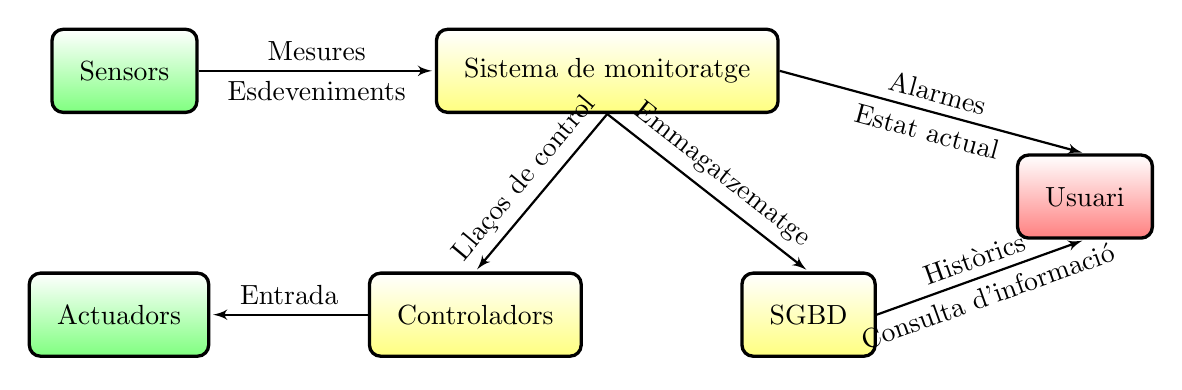
\begin{tikzpicture}[node distance=0.5cm]  
  \tikzset{
    mynode/.style={rectangle,rounded corners,draw=black, 
      very thick, inner sep=1em, minimum size=3em, text centered,
      groc},
    myarrow/.style={->, >=latex', shorten >=1pt, thick},
    mylabel/.style={text width=7em, text centered},
    groc/.style={top color=white, bottom color=yellow!50},
    verd/.style={top color=white, bottom color=green!50},
    roig/.style={top color=white, bottom color=red!50},
  }  

  \node[mynode]                                       (monitor)   {Sistema de monitoratge};  
  \node[mynode, below right=2cm and -0.5cm of monitor]  (bd)        {SGBD}; 
  \node[mynode, below=2cm of monitor, left=2cm and 2cm of bd]     (control)   {Controladors}; 
  \node[mynode, roig, below right=0.5cm and 3cm of monitor] (usuari)    {Usuari};  
  \node[mynode, verd, left=2cm of control]            (actuador)  {Actuadors};
  \node[mynode, verd, left=3cm of monitor]            (sensor)    {Sensors};  


  \draw[myarrow] (monitor.east) --   (usuari.north)	
     node [above,sloped,midway] {Alarmes}
     node [below,sloped,midway] {Estat actual};
  \draw[myarrow] (bd.east) --   (usuari.south)
     node [above,sloped,midway] {Històrics}
     node [below,sloped,midway] {Consulta d'informació};
  \draw[myarrow] (sensor.east) --   (monitor.west) 
     node [above,midway] {Mesures}
     node [below,midway] {Esdeveniments};
  \draw[myarrow] (control.west) -- (actuador.east)
     node [above,midway] {Entrada};
  \draw[myarrow] (monitor.south) -- (bd.north)
     node [above,sloped,midway] {Emmagatzematge};
  \draw[myarrow] (monitor.south) -- (control.north)
     node [above,sloped,midway] {Llaços de control};

\end{tikzpicture} 
  \end{center}
  \caption{Sistema de monitoratge: de l'adquisició de dades fins a informar l'usuari}
  \label{fig:sistema_monitoratge}
\end{figure}


El monitoratge es pot dividir en diferents blocs principals, els quals es mostren a la \autoref{fig:sistema_monitoratge}. Un monitor adquireix dades dels sensors. Les dades poden ser valors de mesures o estats del procés adquirits com a esdeveniments. Fent referència a la classificació de dades temporals de \textcite{assfalg08:thesis}, en general les mesures es poden entendre com a sèries temporals i els esdeveniments com a dades bitemporals.

Per una banda, les dades es poden utilitzar com a sortida del procés en els sistemes de control, els quals calculen els valors d'entrada dels accionaments.
Els llaços de control poden no estar tan centralitzats i habitualment resideixen a prop dels processos que controlen.

Per altra banda, els sistemes de monitoratge informen l'usuari de l'estat actual del procés, tot i que poden només avisar-lo amb alarmes senzilles com per exemple que no s'han pogut adquirir les dades o que el sensor ha disparat un esdeveniment crític. Per a usuari ens referim tant a un usuari humà com a un altre sistema supervisor amb inte\l.ligència artificial. 

Per a càlculs més complicats amb les dades, els sistemes de monitoratge utilitzen sistemes de gestió de bases de dades (SGBD). Mitjançant els SGBD, s'emmagatzemen les dades en bases de dades i posteriorment l'usuari les consulta per observar els històrics o per obtenir informació i descobrir coneixement a partir de les dades emmagatzemades. 

La \autoref{fig:sistema_monitoratge} presenta una visió centralitzada de l'adquisició de dades. Ara bé, els sistemes de monitoratge internament poden tenir estructura distribuïda quan els sensors tenen suficient capacitat de processament, com per exemple les xarxes de sensors. En aquests casos els monitors cedeixen parts al sensors, sobretot pel que fa als SGBD que passen a tenir un paper més rellevant en la comunicació.  







\subsubsection{Problemes en el monitoratge}

Els sistemes de monitoratge habitualment reben problemes derivats de la reco\l.lecció de dades. Principalment distingim tres problemes.

El primer problema és la gestió d'una quantitat enorme de dades. 

Un sistema de monitoratge recull una gran quantitat de dades. Ara bé, l'usuari només en pot observar una petita part sincronitzat (\emph{online}) amb el procés i les dades emmagatzemades esdevenen massa grans per a ser processades posteriorment \parencite{keogh97}. No obstant, les dades han de ser analitzades ja que contenen informació interessant per a les aplicacions de les sèries temporals descrites a l'apartat anterior. S'observa que en el context de monitoratge les dades recollides es poden considerar com a sèries temporals ja que abstractament són una co\l.lecció de mesures.


El segon problema és el de la necessitat de censurar les dades, és a dir validar que les dades siguin correctes i en cas contrari rebutjar-les o reconstruir-les. 

\textcite{quevedo10} mostren la quantitat d'informació que hi ha en els sistemes complexos de telecontrol. Aquesta informació s'obté de diversos sensors distribuïts pel camp de mesura.
En el moment de reco\l.lecció de dades apareixen dos problemes: valors que en un instant de temps prefixat no s'han pogut recollir i valors que són falsos. En el procés de gestió de dades no es poden emmagatzemar les dades amb aquests dos tipus de problema ja que aleshores els registres històrics serien inconsistents. 
Així doncs, cal comprovar que les dades emmagatzemades són correctes, mitjançant un procés de validació, i modificar-les en el cas que siguin falses, mitjançant un procés de reconstrucció que estimi els valors correctes. Per exemple, \citeauthor{quevedo10} apliquen aquests processos de validació i reconstrucció a xarxes de distribució d'aigua.


El tercer problema és dóna quan el període de mostreig no és regular, és a dir que les dades no es recullen de manera uniforme en el temps, però les aplicacions no ho contemplen o volen treballar amb dades a intervals regulars, també anomenat dades equi-espaiades.

Una causa de la irregularitat es deu a que els sistemes de monitoratge informàtics sovint no són capaços de complir amb exactitud el temps de mesura sinó que presenten una certa variació, ja sigui deguda a retards en els sensors, les comunicacions o la planificació del monitoratge amb altres tasques concurrents del sistema operatiu. Aquesta causa, però, es pot atenuar si els sensors envien el temps de mesura juntament amb el valor mesurat. Aleshores, el problema recau en la sincronització dels rellotges dels sensors.

Una altra causa es deu a que l'adquisició de dades prové de processos sotmesos a sistemes de control, els quals prenen el control de l'adquisició de dades. És a dir, el sistema de monitoratge ha d'obeir a les restriccions de temps imposades pels llaços de control. Aquestes restriccions són especialment crítiques en els sistemes de control en temps real ja que, aleshores, el sistema de monitoratge no pot imposar restriccions de temps diferents de les que s'han calculat per als llaços de control.  \textcite{lozoya08} mostren que s'ha de vigilar amb les entrades i sortides de les tasques periòdiques als sistemes en temps real. L'actuació dels sistemes de control es degrada quan no es té en compte que les operacions d'entrada i sortida estan subjectes a fluctuacions degudes al mostreig i a latències. Aquest problema afecta als sistemes de monitoratge en dues vessants.
Per una banda, els sistemes de monitoratge tenen una part de l'adquisició controlada per les aplicacions de control en temps real i per tant el període de mostreig resultant que veu el monitor no és regular. 
Per altra banda, les aplicacions que analitzen les dades obtingudes del monitoratge poden veure com la seva actuació es degrada si no consideren que l'adquisició de dades és irregular, el qual és similar a la regressió que s'observa \parencite{lozoya08} quan en el disseny d'un controlador discret es considera que es mostreja i s'actua periòdicament però en la implementació amb un sistema en temps real aquest pot fluctuar la periodicitat.




En conclusió, per tal de gestionar la complexitat derivada de la recollida de dades i també la complexitat de les consultes posteriors per part de l'usuari, els sistemes de monitoratge es recolzen en sistemes de gestió de bases de dades per gestionar l'emmagatzematge de les dades i la recuperació d'informació.




\subsection{Emmagatzematge i gestió de sèries temporals}


Els sistemes de gestió de bases de dades (SGBD) són els sistemes informàtics que s'encarreguen d'emmagatzemar informació i de permetre a l'usuari consultar-la. A la secció \ref{sec:art:sgbd} es descriu com es formalitzen els SGBD, en aquest apartat ens centrarem en les necessitats que tenen les sèries temporals dels SGBD.


Les sèries temporals es diferencien d'altres tipus de dades en que els seus valors són dependents d'una variable: el temps. Com a conseqüència, qualsevol SGBD que hi vulgui tractar no ho pot fer de manera independent pels valors i pel temps; ha de conservar la coherència temporal.

Per poder aplicar les tècniques d'anàlisis de les sèries temporals de manera eficient cal disposar de SGBD específics. 
Durant l'última dècada, el maquinari informàtic ha millorat tant des del punt de vista tecnològic com de l'econòmic \parencite{deligiannakis07}, el qual ha facilitat l'adquisició de dades, per exemple amb xarxes de sensors, i alhora ha ampliat la capacitat per emmagatzemar les dades. 
Per tant, el volum de dades a tractar  en els SGBD cada cop esdevé més crític.

 
En els SGBD, el problema de grans quantitats de dades també es troba en altres camps com demostren \textcite{mylopoulos96} sobre la necessitat de grans bases de dades de coneixement. Els SGBD que tracten amb aquestes dades s'anomenen \emph{very large databases} (VLDB) i han de construir, accedir i gestionar la quantitat de dades de manera eficient.

\textcite{ogras06}  consideren que les solucions de les VLDB estan pensades per a bases de dades estàtiques. No obstant, observen que les sèries temporal normalment són dinàmiques, és a dir de naturalesa contínua i de mida no fitada. Conseqüentment, conclouen que les solucions tradicionals no es poden aplicar a causa de l'arribada seqüencial de les dades i que no es poden processar aleatòriament. 
Com a solució proposen resumir dinàmicament les sèries temporals amb les tècniques de compressió que s'apliquen en altres aplicacions on hi ha bases de dades grans.




\textcite{dreyer94} proposen desenvolupar SGBD que implementin operacions específiques per les sèries temporals, aleshores els anomenen sistemes de gestió de bases de dades per sèries temporals (SGST, \emph{time series database management systems}). Consideren que els altres SGBD no són adequats per tractar sèries temporals, tot i que després de comparar els SGBD per dades temporals i els SGST \parencite{schmidt95} troben que hi ha aspectes comuns entre els dos sistemes.
Els SGST estan optimitzats per gestionar les dades segons les operacions de temps i rotació, les quals són molt comunes en la gestió de les sèries temporals.  A més també cal controlar el creixement de la base de dades i la consulta ha de ser flexible i d'alta velocitat \parencite{keogh10:isax}. 
No obstant, fins a on coneixem, les propietats d'un model de SGST no s'han investigat més enllà  ja que la recerca s'ha concentrat en tasques de mineria de dades. Per exemple \textcite{last01} estudien una metodologia general per descobrir coneixement en els SGST, tant pel que fa a 
patrons temporals %(groups of events ordered by time)
com a regles temporals%(cause-effect relationships between events)
, i breument noten l'existència del model \cite{dreyer94} pels SGST.


Altres estudis proposen tractar les sèries temporals com a tipus que tenen ordre, per exemple seqüències o matrius.

\textcite{seshadri96:thesis} proposa que les sèries temporals són un subconjunt de les seqüències i per tant el model i les operacions per les seqüències \parencite{seshadri95} serveixen per les sèries temporals. 
\textcite{bonnet01} utilitzen el model de seqüències en SGBD distribuïts per xarxes de sensors, aleshores l'estratègia de comunicació inclou agregacions de les sèries temporals en els sensors \parencite{demers03}.
També es relaciona el model de seqüències de les sèries temporals amb els \emph{data streams} \parencite{babcock02,jagadish95}. Els \emph{data streams} són dades que arriben contínuament i amb ordre temporal i es modelen com una seqüència on només s'hi poden afegir elements. Aleshores les consultes poden ser contínues, és a dir cada cop que arriba una dada nova s'actualitza incrementalment la informació. Per les sèries temporals s'utilitza en el càlcul de correlacions i prediccions de forma incremental \parencite{yi00} i en la cerca de patrons \parencite{bai05}.
%Data Stream Management System (DSMS) is an extension of Data Base Management System  

En els SGBD per matrius \emph{arrays} destaquen els anomenats sistemes de gestió de bases de dades científiques, camp en el qual les sèries temporals hi tenen un paper de primer ordre \parencite{zhang11}. \textcite{stonebraker09:scidb} estudien les necessitats d'aquests sistemes sobretot en l'àmbit de la ciència. \textcite{kersten11} proposen un sistema molt semblant però a més integren el seu llenguatge, anomenat SciQL, amb la sintaxi de SQL. \textcite{zhang11} exemplifiquen detalladament l'ús de SciQL per a les sèries temporals per a algunes de les seves propietats: regularitat, interpolació i cerca de correlacions.



\subsubsection{Implementacions actuals}

Hi ha hagut implementacions de sistemes específics per a sèries temporals. Alguns són només l'aplicació d'un algoritme d'anàlisi per un problema concret de sèries temporals però  altres  són més elaborats i es defineixen com a SGBD per a sèries temporals. 
En aquest apartat resumim algunes aplicacions que considerem que implementem conceptes dels SGST.


\paragraph{Calanda} \textcite{dreyer94} proposen els requeriments de propòsit específic que han de complir els SGST i basen el model en quatre elements estructurals bàsics: esdeveniments, sèries temporals, grups i metadades, a banda de les bases de dades per sèries temporals. Implementen un SGST anomenat Calanda \parencite{dreyer94b,dreyer95,dreyer95b} que té operacions de calendari, pot agrupar sèries temporals i respondre consultes simples i ho exemplifiquen amb dades econòmiques. A \cite{schmidt95} es compara Calanda amb els SGBD temporals que operen amb sèries temporals. 




\paragraph{T-Time}  \textcite{assfalg08:thesis} mostra un sistema que pot cercar similituds calculades com a distàncies entre sèries temporals. Principalment, dues sèries temporals es marquen com a similars si la seva distància és menor que un llindar en cada interval. A partir d'aquest mètode dissenya algoritmes eficients que implementa en un programa anomenat T-Time \parencite{assfalg08:ttime}.


 
\paragraph{iSAX} \textcite{keogh08:isax,keogh10:isax} estudien l'anàlisi i l'indexat de co\l.lecions massives de sèries temporals. Descriuen que el problema principal del tractament rau en l'indexat de les sèries temporals i proposen mètodes per calcular-lo de manera eficient. El mètode principal que proposen està basat en l'aproximació a trossos constants de la sèrie temporal \parencite{keogh00}.  Ho implementen en una estructura de gestió de dades que anomenen \emph{indexable Symbolic Aggregate approXimation} (iSAX) \parencite{isax}. Les representacions de sèries temporals que s'obtenen amb aquesta eina permeten reduir l'espai emmagatzemat i indexar tant bé com altres mètodes de representació més complexos.




\paragraph{TSDS} \textcite{weigel10} noten la necessitat de mostrar les dades en tot el seu rang temporal i no només en un subconjunt com normalment s'ofereixen. Desenvolupen el paquet informàtic \emph{Time Series Data Server} (TSDS) \parencite{tsds} a on es poden introduir les dades de sèries temporals per posteriorment consultar-les per rangs temporals o aplicant-hi filtres i operacions.





\paragraph{RRDtool} RRDtool \parencite{rrdtool} {é}s un SGBD molt usat per la comunitat de programari lliure. Projectes en diversos camps l'utilitzen com a SGBD, en els quals hi ha sistemes de monitoratge professionals, també en l'àmbit de programari lliure, com Nagios/Icinga \parencite{nagios,icinga} o el Multi Router Traffic Grapher (MRTG) \parencite{mrtg}. Aquests monitors transfereixen a RRDtool la responsabilitat de gestionar l'emmagatzematge i d'operar amb les dades, i així es poden centrar en l'adquisició de dades i la gestió d'alarmes. 
En l'evolució de RRDtool hi ha dues millores destacables. En primer lloc, \textcite{lisa98:oetiker} va separar el sistema de gestió de RRDtool de MRTG i el va dissenyar amb una estructura característica de Round Robin. En segon lloc,  \textcite{lisa00:brutlag} va estendre RRDtool amb algoritmes de predicció i detecció de comportaments aberrants. 
Actualment, s'està estudiant l'eficiència i rapidesa de RRDtool a processar sèries temporals. \textcite{carder:rrdcached} ha dissenyat una aplicació, \emph{rrdcached}, que millora el rendiment de RRDtool amb la qual s'aconsegueix fer funcionar  simultàniament sistemes amb grans quantitats de bases de dades RRDtool \parencite{lisa07:plonka}. \textcite{jrobin} han dissenyat una adaptació de RRDtool anomenada \emph{JRobin}. 
Finalment, és destacable l'ús emergent de RRDtool en entorns d'experimentació, com és el cas de \textcite{zhang07} i \textcite{chilingaryan10} que hi emmagatzemen dades experimentals per posteriorment predir o validar-les.


\paragraph{Cougar} \textcite{cougar} proposen Cougar com un SGBD per xarxes de sensors (\emph{sensor database systems}). El sistema té dues estructures \parencite{bonnet01}: una basada en relacions per les característiques dels sensors i una basada en seqüències per les dades dels sensors, les quals són sèries temporals.
Les consultes es processen de manera distribuïda: cada sensor és un node amb capacitat de processament que pot resoldre una part de la consulta i fusionar-la amb les altres. D'aquesta manera es minimitza l'ús de comunicacions però l'estructura i estratègia de comunicació dels nodes esdevé una part crítica a configurar \parencite{demers03}.

\paragraph{TinyDB} Un altre prototip de SGBD per xarxes de sensors desenvolupat para\l.lelament a Cougar és TinyDB \parencite{tinyDB}. A part de les característiques descrites per Cougar, aquest sistema  modifica i s'implica en parts del procés d'adquisició de les dades com és el temps, la freqüència o l'ordre de mostreig. Per exemple donada una consulta que vol correlacionar les dades de dos sensors, el sistema indica als sensors implicats que han d'adquirir amb la mateixa freqüència.

\paragraph{SciDB} \textcite{stonebraker09:scidb} estudien els SGBD científiques amb models  de dades basats en matrius. Estan desenvolupant SciDB \parencite{scidb}, un SGBD productiu i optimitzat per treballar amb matrius.


\paragraph{SciQL} \textcite{kersten11} descriuen SciQL, un llenguatge per a SGBD científiques. Hi ha un prototip en desenvolupament de SciQL \parencite{sciql}.





\subsection{Visió general}

Els SGST actuals bàsicament resolen alguns problemes d'anàlisis de sèries temporals.
Però no solen atendre la relació entre la base de dades i el sistema de monitoratge, és a dir la manera com s'adquireixen les dades. En aquest pas intermig hi ha un sèrie de problemes, com per exemple forats, dades falses o irregularitat en els temps de mostreig, que cal gestionar correctament. Concretament un dels problemes que no s'atén és el de mostreig irregular ja que es considera que les mostres estan a intervals regulars (equi-espaiades) encara que els sistemes de monitoratge informàtics sovint no són capaços de complir-ho amb exactitud sinó que presenten una certa variació en els temps de mesura. 

RRDtool n'és una excepció ja que, per ser un sistema productiu, el processament de dades i emmagatzematge és més proper als sistemes de monitoratge. No obstant, està centrat en un tipus de dades particulars, les magnituds i els comptadors, i no té tantes operacions generals per les sèries temporals com els altres SGST.

També Cougar i TinyDB que exploren l'encaix dels SGBD en entorns distribuïts de xarxes de sensors. Proposen noves estratègies de comunicació amb l'objectiu d'ajustar el consum d'energia. 


SciQL, un model recent per SGBD  basat en matrius, és el que més es pot considerar com a SGST, ja que s'està desenvolupant per complir-ne algunes propietats.



%%% Local Variables: 
%%% mode: latex
%%% TeX-master: "main"
%%% End: 

% LocalWords:  monitoratge



\section{Sistemes de gestió de bases de dades}
\sectionmark{SGBD}
\label{sec:art:sgbd}


Segons \textcite{date:introduction}, ``una base de dades és un
contenidor informàtic per a una co\l.lecció de dades''. El sistemes
informàtics que tracten amb bases de dades s'anomenen sistemes de
gestió de bases de dades (SGBD, \emph{Data Base Management Systems}) i
tenen els objectius d'emmagatzemar informació i permetre consultar i
afegir aquesta informació per part dels usuaris.  Per complir aquests
objectius, els SGBD ofereixen a l'usuari diferents operacions com per
exemple crear una base de dades, afegir dades o consultar informació a
partir de les dades emmagatzemades.

Els SGBD es poden descriure mitjançant teories matemàtiques que reben
el nom de model de dades, per tant es poden veure els SGBD com una
implementació d'un model de dades.  Segons
\citeauthor{date:introduction}, ``un model de dades és una definició
abstracta, auto continguda i lògica dels objectes, de les operacions i
de la resta que conjuntament constitueixen la màquina abstracta amb la
que els usuaris interaccionen. Els objectes permeten modelar
l'estructura de les dades. Les operacions permeten modelar el
comportament''. Ara bé, \citeauthor{date:introduction} avisa que el
concepte model de dades també s'usa per a definir una estructura
persistent de dades concreta i, per tant, cal distingir adequadament
entre els dos conceptes.  Tal com fa Date, en aquest document parlarem
de model de dades, o simplement de model, en el primer sentit de
màquina abstracta.


Un model de SGBD que ha s'ha consolidat i esdevingut un referent és el
model relacional (\emph{relational}). L'èxit d'aquest model és degut a
que es fonamenta en teories matemàtiques consolidades: la lògica de
predicats i la teoria de conjunts \parencite{date:introduction}.



\textcite{date:introduction} diferencia amb detall els conceptes de
model i d'implementació.  El model d'un SGBD és el model matemàtic tal
com s'ha descrit anteriorment, en canvi un SGBD és la implementació
d'un model de dades, per exemple \emph{PostgreSQL} \parencite{postgresql}.
%Segons l'esquema de comunicació, també es poden anomenar com a sistema servidor de bases de dades, per exemple postgresql.
En aquest context una base de dades és una instància d'un SGBD,
per exemple la base de dades dels estudiants.


Aquesta diferència entre implementació i model aporta independència de dades (\emph{data independence}) \parencite{date:dictionary}. En altres paraules, els models no han de tenir detalls d'implementació ni parlar d'objectius de rendiment. 
\textcite{dbdebunk} detallen algunes confusions actuals sobre la independència entre el model i la implementació.







\subsection{Sistemes relacionals}
\label{sec:estat:sgbdr}

El model relacional va ser proposat per \textcite{codd70} per a
formalitzar els SGBD, els quals quan es basen en aquestes teories
s'anomenen relacionals (SGBDR). A partir de llavors els SGBDR han anat
evolucionat fins a aconseguir una gran solidesa, amb
\textcite{date:introduction,date06,date:dictionary} com a principal
divulgador.



Les implementacions més populars de SGBDR són les que s'anomenen
\emph{SQL} ja que tenen en comú el llenguatge \emph{Structured Query
  Language}. Ara bé, els SGBD \emph{SQL} es desvien considerablement
del model relacional: permeten files duplicades, tenen ordre en les
columnes, permeten valors nuls, etc, sent aquest últim un tema
actualment discutit \parencite{date08:nulls}.

Les diferències entre els SGBD \emph{SQL} i el model relacional han
contribuït a que hi hagi hagut una sèrie de malentesos i
errors, alguns dels quals han estat avaluats i desmentits per
\citeauthor{dbdebunk} en vàries
publicacions \parencite{dbdebunk,date06}.
  

\textcite[cap.~2]{date06} %ch2pp21-22
considera que no hi cap implementació comercial que segueixi fidelment
el model relacional, tot i que esmenta algunes implementacions
prometedores com \emph{Dataphor} o la seva proposta tecnològica
\emph{TransRelational} \parencite{date:transrelational}. A banda,
també cal destacar \emph{Rel} \parencite{rel} com un SGBDR bastant
consolidat.



Actualment \textcite{date:thethirdmanifesto} estan treballant en el
'\emph{Third Manifesto}' com a proposta per a obtenir SGBDR purament
relacionals. Destaquen que, en el model relacional, els tipus de dades
i les relacions són necessaris i suficients per representar qualssevol
dades a nivell lògic. %[date06ch21,369]
Defineixen dos principis bàsics dels SGBDR: l'\emph{Information
  Principle} o \emph{The Principle of Uniform
  Representation} \parencite{date:dictionary}, segons el qual una base
de dades només conté variables relacions, i el principi
d'ortogonalitat entre la teoria de tipus i el model
relacional \parencite[cap.~6]{date06}, segons el qual relacions i
tipus de dades són independents i per tant els atributs de les
relacions admeten qualsevol tipus.  Segons aquest punt de vista, els
tipus de dades són el conjunt de coses de les que podem parlar mentre que les
relacions són proposicions certes sobre aquestes coses.
%In other words, types give us our vocabulary the things we can talk about and relations give us the ability to say things about the things we can talk about. (There's a nice analogy here that might help: Types are to relations as nouns are to sentences.) %[date05ch4secMore on Relations Versus Types]

En la proposta per a obtenir SGBDR purament relacionals
\textcite{date06:_datab_types_relat_model,date:tutoriald} classifiquen
com a \emph{D} els llenguatges que segueixin els principis del
\emph{Third Manifesto}. Concretament, com a exemple d'un llenguatge
\emph{D} estan definint les regles de \emph{Tutorial D}, que ha de
servir pels estudis del model relacional a nivell acadèmic. Aquest
llenguatge ja s'utilitza en alguns SGBDR, com per exemple a
\emph{Rel} \parencite{rel}.


El model relacional ha incorporat conceptes d'altres disciplines. En
destaca sobretot la incorporació de conceptes dels models d'orientació
a objectes com és el cas de l'herència.  Aleshores s'entén que els
SGBDR també es puguin anomenar SGBD objecte/relacionals
(\emph{object/relational})
\parencite{date02:foundation}.  Tot i així, \textcite[cap.~6]{date06}
manifesta i avisa de l'ús de la mateixa terminologia amb significat
diferent entre el model relacional i l'orientació a objectes, sobretot
pel que fa als termes valor i variable. %[date06ch6pp91]
La seva hipòtesi a aquestes diferències és que el model relacional és
un model de dades i el model d'orientació a objectes és més proper a
un model
d'emmagatzematge. % 'the object model' is closer to being a model of
                  % storage than it is to being a model of
                  % data. [date06ch6pp92]

% A la \autoref{tab:sgbd:relacional-objectes} es resumeix la possible
% equivalència lògica dels conceptes entre el model relacional i
% l'orientació a objectes tal com Date exposa al capítol 6, tot i que
% cal tenir en compte que la semblança és difusa.

% \begin{table}
% \centering
% \begin{tabular}[ht]{ll}
%   relacional & objectes \\\hline \hline
%   tipus & tipus, classe, interfície \\\hline
%   representació & classe, atributs, propietats \\\hline
%   valor, objecte, instància & valor, estat, objecte/instància immutable/estàtic \\\hline
%   variable & valor, objecte/instància mutable/dinàmic \\\hline
%   referència & variable \\\hline
%   operador & funció, mètode \\\hline
% \end{tabular}
% \caption{Possible equivalència lògica de termes entre el model relacional i l'orientació a objectes \parencite[cap.~6]{date06}.}
% \label{tab:sgbd:relacional-objectes}
% \end{table}

% Relacional: tipus | representació |  valor, objecte, instància  | variable  | referència (adreça continguda en una variable) | operadors (de lectura i de modificació)
% Objectes: tipus, classe (tipus amb atributs i mètodes), interfície | classe, atributs,propietats  |  valor, estat, objecte/instància immutable/estàtic |  valor, objecte/instància mutable/dinàmic  | variable | funcions,mètodes (funcions dins de classes) (purs o modificadors)



\subsubsection{Extensió del model}
%Com s'ha d'estendre el model relacional?

El model relacional ha evolucionat però no es considera que hi hagi hagut
cap revolució des de la seva aparició
\parencite[cap.~19]{date06}. %[date06ch19pp254]
Consideren que el model relacional és bastant complet i que segueix
evolucionant en la comprensió de les teories i els conceptes que hi
intervenen, com per exemple la recent àlgebra relacional
'A' \parencite[ap.~A]{date06:_datab_types_relat_model}.  En aquest
context d'evolució, es contemplen les investigacions que poden
estendre el model relacional, és a dir, aconseguir abstraccions més
generals de les dades \parencite[cap.~25]{date06}. %[date06ch25pp441]

% En l'extensió hi ha el què després s'aplica a sobre: optimitzacions,
% redundàncies, etc.

En el sentit d'extensió, també cal contemplar la definició de nous
tipus de dades, els quals estenen els SGBD en funcionalitat.  Aquests
nous tipus de dades poden afegir estructures i operadors que ja siguin
expressables amb l'àlgebra relacional. No obstant, un bon model d'un
tipus de dades serveix per augmentar el nivell d'abstracció en el
tractament dels conceptes relacionats amb aquestes
dades
\parencite{date02:_tempor_data_relat_model}. %[date02:_tempor_data_relat_model:prefaceppxix]

Com s'ha dit anteriorment, la teoria de tipus i el model relacional
són ortogonals: el model relacional requereix que hi hagi un 'sistema'
de tipus de dades però diu molt poc de la naturalesa d'aquest sistema,
si bé el model relacional defineix que com a mínim hi ha d'haver el
tipus booleà i el tipus
relació \parencite{date:thethirdmanifesto}. Pel que fa a implementar
el tipus de dades en els SGBD, els quals aleshores també s'anomenen
SGBD objecte/relacionals, destaquen les primeres propostes fetes per
\textcite{stonebraker86} per tal que els usuaris puguin definir els
seus propis tipus de dades i les de \textcite{seshadri98:_enhan} que
estudia la definició de tipus de dades complexos per tal que es puguin
tractar eficientment.

\todo{ampliació de tipus als SGBD molt important a GIS [bollaert06:thesis]}

 




\subsection{Altres sistemes}

Les crítiques als SGBDR, sobretot les degudes als SGBD
\emph{SQL}, han contribuït a voler explorar altres models de
SGBD \parencite{stonebraker09}. Aquests models presenten diferents
maneres de representar les dades: llistes, seqüències, enllaços,
matrius, etc.
%[date06pp116,134]

Tot i així, \textcite[cap.~21--25]{date06} considera que els nous
models de SGBD, a vegades anomenats post-relacionals, no estan fundats
tant sòlidament en teories matemàtiques i la lògica de predicats com
el model relacional i pronostica que ens els propers cent anys els
SGBD encara estaran basats en el model
relacional. %[date06ch19pp354,date06ch20pp365]
Considera la possibilitat, tot i que remota, que es pugui definir un
model més potent que el relacional però que no hi ha cap indici que
cap definició dels nous model tingui la mateixa potència que el
relacional. Per tant, aconsella que per ara els SGBD no s'allunyin del
model relacional. %[date06ch25,ch21pp379-380]




Recentment ha aparegut un nou corrent en l'àmbit dels SGBD que
s'anomena NoSQL (\emph{Not Only SQL}) amb l'objectiu de sobrepassar
les limitacions dels SGBDR \parencite{edlich:nosql,stonebraker10}.  A
l'espera que Date valori aquest corrent, cal tenir present els seus
apunts sobre sistemes relacionals contra sistemes no
relacionals \parencite[part 7]{date06}, sobretot pel que fa al
concepte de l'\emph{Information Principle} i que SQL no és un bon
referent pels SGBDR. És a dir, s'ha d'entendre NoSQL com una crítica a
les implementacions comercials actuals del model relacional, una
crítica que pot estar motivada per l'ús de SQL per part d'aquest
productes.  No es pot entendre, però, el NoSQL com una crítica al
model relacional ja que els objectius parlen de millorar el rendiment
dels SGBD, cosa només atribuïble a les implementacions però no al
model. Precisament, actualment del model relacional destaca la
proposta de \citeauthor{date:tutoriald} d'un llenguatge,
\emph{Tutorial D}, que no és SQL.


El corrent de NoSQL també critica l'adequació dels productes actuals.
Els SGBD NoSQL apunten els SGBDR actuals per voler ser \emph{one size
  fits all} \parencite{stonebraker07,stonebraker09} però que cada
aplicació té els seus requisits i per tant una mateixa implementació
no pot ser bona per a tots el camps.  En aquesta mateixa línia els
models pels SGBD prenen més sentit que mai ja que permeten mantenir
una definició comuna per a moltes implementacions.


Segons es desprèn de \textcite{date06} fins a l'actualitat només hi ha
hagut un model consolidat pels SGBD: el model relacional.  Ara, en el
corrent NoSQL també es parla de nous models de
SGBD \parencite{edlich:nosql,stonebraker09:scidb}.
\citeauthor{date06} ha avaluat que alguns nous models recuperen
intents fallits en el passat tot i que es poden representar amb el
model relacional, per exemple els SGBD XML basats en estructures
d'arbre \parencite[cap.~14]{date06} \parencite[cap.~27]{date04:introduction8}
o els ODMG basats en objectes \parencite[cap.~27]{date06}. Tot i així,
en un futur cal estar atents per si alguns d'aquests models joves de
SGBD arriben a consolidar-se i poden esdevenir tant potents com el
model relacional.





\subsection{Dades temporals}

%parlar de docs anteriors de dades temporals

%Precisament,
Una de les extensions importants del model relacional s'ha produït amb
l'estudi de les dades
temporals \parencite{date02:_tempor_data_relat_model}. Amb el model de
dades temporals basat en el model relacional s'obtenen SGBDR capaços
d'emmagatzemar i consultar dades històriques.

El model de les dades
temporals \parencite{date02:_tempor_data_relat_model} es basa en
relacions i intervals per representar les dades històriques. Cada
relació s'estén amb un atribut que és un interval temporal que indica
el rang temporal de validesa de les proposicions. A més el model també
defineix les operacions necessàries per tractar amb les dades
temporals. Aquestes operacions són extensions de l'àlgebra relacional.
El principal objectiu del model de dades temporals és poder tenir
suport per a les dades històriques en els SGBDR.
\textcite[cap.~28]{date06} compara aquest model per dades temporals
amb altres aproximacions que s'han fet no basades en el model
relacional.



El model de dades temporals representa les dades històriques amb el
temps vàlid i temps de
transacció \parencite[cap.~15]{date02:_tempor_data_relat_model}, el
que es coneix com a dades bitemporals.  Així doncs, els SGBD per dades
bitemporals no es consideren adequats com a SGBD per sèries temporals
ja que els primers estan pensats per a històrics, es descriuen amb
intervals temporals, i els segons per anàlisi d'observacions
seqüencials, es descriuen amb instants temporals.
\textcite{schmidt95} arriben a aquesta conclusió després de comparar
els SGBD bitemporals amb els de sèries temporals, tot i que per a
desenvolupaments futurs observen que hi aspectes temporals comuns
entre els dos sistemes i es pregunten si es podran trobar sistemes que
els englobin a tots dos o cadascun necessitarà sistemes específics.


%a algun lloc deia Date que el seu model per dades temporals no era del tot adequat per les sèries temporals?, potser perquè els intervals no estaven pensat per a instants? date02ch16.8?



\subsection{Conclusió}


Actualment l'àmbit informàtic de SGBD se centra en les
implementacions, com ho demostra el nou corrent NoSQL concentrat en
trobar models d'implementacions que tinguin bon rendiment. A tal
efecte la recerca es concentra en temes de garantia de propietats ACID
(\emph{atomicity, consistency, isolation, durability}), d'optimització
de consultes, d'emmagatzematge de grans volums de dades, de consultes
via web, de distribució de bases de dades, de reduir la despesa en
energia, etc. \parencite{stonebraker07,stonebraker10}, la qual cosa és
exce\l.lent per a disposar d'un SGBD adequat a cada aplicació.
\textcite{haerder05:_dbms_archit} descriu diferents models
d'implementació per als SGBD, ja que indica que per obtenir bon
rendiment la implementació d'un SGBD s'ha d'estudiar per cada
aplicació. És més, una implementació d'un SGBD que vulgui obtenir un
bon rendiment en una determinada aplicació potser no pot implementar
el model de dades complet sinó que només una part, com per exemple en
els sistemes
encastats \parencite{saake09:_downs_data_manag_embed_system}.

Per altra banda, l'àmbit matemàtic de SGBD, amb el model relacional
com a màxim exponent, se centra en els conceptes teòrics, és a dir
respon a la pregunta de què són els SGBD. Recerca en millorar-ne la
comprensió, en obtenir la màxima potència i facilitat de cara a la
gestió de dades per part de l'usuari o en obtenir nous models. Tot i
així, actualment encara no s'ha trobat cap altre model que tingui la
mateixa potència que el relacional. Cal destacar que tot i que el
model relacional té conceptes madurs i consolidats, i que a més han
tingut èxit amb els SGBD SQL, s'obre una nova perspectiva amb
l'evolució de conceptes que proposa el \emph{Third Manifesto},
especialment amb \emph{Tutorial D} i les implementacions que comencen a prendre
cos a nivell acadèmic.



















%%% Local Variables: 
%%% mode: latex
%%% TeX-master: "main"
%%% End: 

% LocalWords:  monitoratge SGBD SGBDR






%%% Local Variables: 
%%% mode: latex
%%% TeX-master: "main"
%%% End: 

% LocalWords:  monitoratge
